% Editable native PGFPlots figure. Four user-specified PSD points.
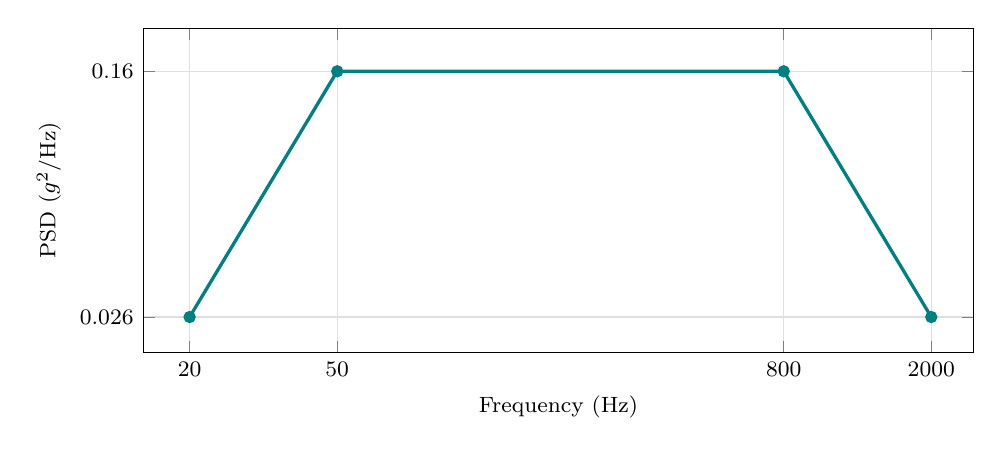
\begin{tikzpicture}
\begin{loglogaxis}[
 width=\linewidth,height=5.7cm,
 xmin=15,xmax=2600,ymin=0.02,ymax=0.22,
 xlabel={Frequency (Hz)},ylabel={PSD ($g^2$/Hz)},
 xtick={20,50,800,2000},xticklabels={20,50,800,2000},
 ytick={0.026,0.16},yticklabels={0.026,0.16},
 grid=both,major grid style={gray!25},minor grid style={gray!12},
 tick label style={font=\footnotesize},label style={font=\footnotesize},
 scaled ticks=false]
\addplot[color=Teal,line width=1.2pt,mark=*,mark size=1.6pt]
 coordinates {(20,0.026) (50,0.16) (800,0.16) (2000,0.026)};
\end{loglogaxis}
\end{tikzpicture}
